\documentclass[a4paper,12pt,twocolumn,landscape]{article}

\usepackage{superpack2015}
\usetikzlibrary{decorations.fractals}

\usepackage[heightrounded]{geometry}	% heightrounded permet d'afficher les footers correctement
\geometry{hmargin=0.5cm,vmargin=1.5cm}

\setlength{\columnseprule}{0.5pt}		% Ligne séparatrice milieu document
\setlength{\columnsep}{50pt}			% Espace de chaque côté de la ligne
\setlength{\headsep}{15pt}
\addtolength{\textheight}{20pt}
%\setlength{\textwidth}{770pt}
%\setlength{\hoffset}{20pt}

\classichf
	% Nom du style
	{sujet}
	% Hauteur sous header
	% 14.5pt si une ligne (1 \baselineskip)
	% 29.0pt si deux lignes (2 \baselineskip)
	{14.5pt}
	% Head
	{}
	{\textbf{Exercices : Généralités sur les fonctions}}
	{}
	% Foot
	{}
	{}
	{}

%\usepackage{showframe}
%\usepackage{layout}

\newcommand{\courbeVonKoch}[1]{
\begin{tikzpicture}[decoration=Koch snowflake]
	\draw[scale=#1]	decorate{decorate{decorate{decorate{decorate{(0,0) -- (1,0)}}}}};
\end{tikzpicture}
}
\newcommand{\floconVonKoch}[1]{
\begin{tikzpicture}[decoration=Koch snowflake]
	\draw[scale=#1]	decorate{decorate{decorate{decorate{decorate{(0,0) -- (1,0) --++ (-120:1) --++ (-240:1)}}}}};
\end{tikzpicture}
}

\begin{document}
\pagestyle{sujet}	%\thispagestyle{premierepage} pour isoler des styles de pages

\exercice On considère le quadrilatère tournant vu à l'activité~1~:\\[1em] \noindent
$ABCD$ représente une feuille au format~$A4$ c'est-à-dire un rectangle de côtés $AB = 29,7cm$ et $BC = 21cm$.\\
On place $M$ sur $[AB]$.\\
On place ensuite $N$ sur $[BC]$, $P$ sur $[CD]$ et $Q$ sur $[DA]$ tels que~:\\ $AM = BN = CP = DQ$\\[1em]
On pose $x$ la longueur $AM$.\\[1em]
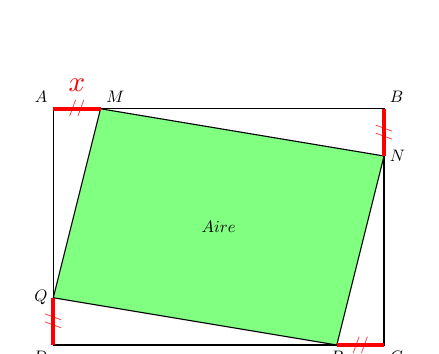
\begin{tikzpicture}[scale=0.6,every node/.style={scale=0.6}]
	\coordinate (A) at (0,0);
	\coordinate (B) at (7,0);
	\coordinate (C) at (7,-5);
	\coordinate (D) at (0,-5);
	\coordinate (M) at (1,0);
	\coordinate (N) at (7,-1);
	\coordinate (P) at (6,-5);
	\coordinate (Q) at (0,-4);
	\coordinate (S) at (7/2,-5/2);
	\draw (A) rectangle ++(7,-5);
	\draw (A)--(B)--(C)--(D)--cycle;
%	\draw [very thick,red] (A)--(M) node [midway,above] {$x$};
	\draw [black,fill=green!50] (M)--(N)--(P)--(Q)--cycle;
	\draw (A) node[above left] {$A$};
	\draw (B) node[above right] {$B$};
	\draw (C) node[below right] {$C$};
	\draw (D) node[below left] {$D$};
	\draw (M) node[above right] {$M$};
	\draw (N) node[right] {$N$};
	\draw (P) node[below] {$P$};
	\draw (Q) node[left] {$Q$};
	\draw (S) node {$Aire$};
%	\foreach \point in {A, B, C, D}
%		\draw (\point) node[above left] {$\point$};
	\draw [red,ultra thick] (A)--(M)node[midway,sloped]{$//$};
	\draw [red,ultra thick] (B)--(N)node[midway,sloped]{$//$};
	\draw [red,ultra thick] (C)--(P)node[midway,sloped]{$//$};
	\draw [red,ultra thick] (D)--(Q)node[midway,sloped]{$//$};
	\draw (0.5,0.5) node [scale=1.75,red] {$x$};
\end{tikzpicture}
\\[1em]
\begin{enumerate}
	\item Montrez que l'aire verte peut s'écrire comme une fonction de $x$ dont on précisera le domaine de définition. On note cette fonction~$f$ et on a $f(x) = 2x^2 - 50,7x + 623,7$
\end{enumerate}
%\begin{tikzpicture}[scale=0.5,yscale=3,every node/.style={scale=0.7}]
\tkzInit[xmax= 22,xstep=1,ymax=3,ystep=1]
\tkzGrid[sub]
\tkzDrawX[label={\textit{heure le 28/10/2015}},above left=18pt,fill=white]
\tkzLabelY
\tkzLabelX
\tkzDrawY[label={\textit{hauteur d'eau du Gardon d'Al\`es}},below right=18pt]

\draw plot[smooth] file {ales.table};
\end{tikzpicture}
%\input{fonctions1-exercice3}

\courbeVonKoch{6}
\floconVonKoch{6}


\begin{tikzpicture}[scale=1,every node/.style={scale=1}]

\foreach \pos/\y in {1/10,2/20,3/30,4/40,5/50,6/60,7/70,8/80,9/90,10/100}
\fill[color=blue!\y](\pos,0) circle (0.5cm) ;


\end{tikzpicture}

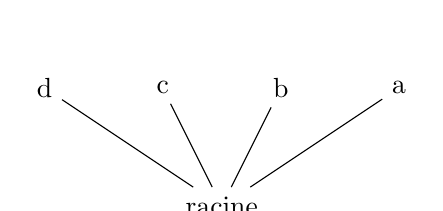
\begin{tikzpicture}[scale=1,every node/.style={scale=1}]

\node {racine}[grow=up] child foreach \name in {a,b,c,d} {node {\name}} ;

\end{tikzpicture}

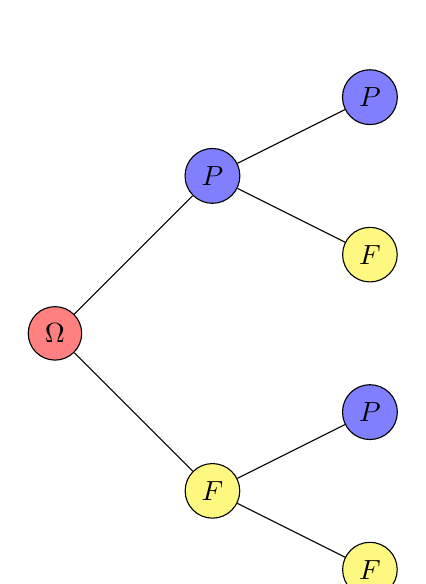
\begin{tikzpicture}[scale=1,every node/.style={scale=1}]
\tikzstyle{omega}=[circle,draw,fill=red!50]
\tikzstyle{face}=[circle,draw,fill=yellow!50]
\tikzstyle{pile}=[circle,draw,fill=blue!50]
\tikzstyle{espaces}=[level 1/.style={level distance=2cm,sibling distance=4cm},level 2/.style={level distance=2cm,sibling distance=2cm}]

\node[omega] {$\Omega$} [espaces,grow=right]
child {node[face] {$F$}
child {node[face] {$F$}}
child {node[pile] {$P$}}}
child {node[pile] {$P$}
child {node[face] {$F$}}
child {node[pile] {$P$}}
};
\end{tikzpicture}


%\begin{tikzpicture}[decoration=Koch snowflake]
%	
%\foreach \x in {1, ..., 3}
%	\draw[scale=\x]	decorate{
%					decorate{
%					decorate{
%					decorate{
%					(0,0) -- (1,0) --++ (-120:1) --++ (-240:1)
%					}
%					}					}
%					};
%\end{tikzpicture}

\end{document}


%
%%\exercicebareme{4}
%\exercicebareme{6}
%\exercicebareme{10}
%\exerciceunpoint
%\exercicebonus
%\FIN
%\BONNESVACANCES
%\BONCOURAGE
%\hrulefill